\chapter{Native mass spectrometry reveals the structural basis of distinct ligand modes of action.}
\label{chapter:mass_spec}

\section{Introduction}
The oligomeric state adopted by PKM2, and how ligand binding affects changes to the monomer-dimer-tetramer equilibrium, remains controversial. PKM2 forms a homotetrameric complex in crystal structures, both in the absence and in the presence of various co-crystalised allosteric ligands and substrates \cite{Anastasiou:2012aa,Chaneton:2012aa,Christofk:2008aa,Dombrauckas:2005aa,Morgan:2013aa,Yuan:2018aa}. Solution-phase chromatographic measurements of PKM2 size, however, have shown that PKM2 forms an equilibrium of monomers and tetramers \cite{Anastasiou:2012aa,Hofmann:1975aa,Kato:1989aa,Morgan:2013aa,Yuan:2018aa}, with some studies reporting the existence of dimers \cite{Keller:2012aa,Yan:2016aa}, in which the tetramer has high enzymatic activity whereas monomers and dimers display lower levels of activity \cite{Anastasiou:2012aa,Ashizawa:1990aa,Ashizawa:1991aa,Hofmann:1975aa,Mazurek:2011aa}. Accordingly, the regulation of PKM2 oligomerisation by various allosteric ligands in solution \cite{Anastasiou:2012aa,Ashizawa:1990aa,Hofmann:1975aa,Keller:2012aa,Morgan:2013aa,Yan:2016aa,Yuan:2018aa} and in the gas phase \cite{Gavriilidou:2018aa}, has been previously reported as a mechanism by which PKM2 activity can be modulated. In addition to oligomerisation, several studies of PKM2 and its homologues have implicated ligand-induced conformational changes as contributing to the inactive-active state transition \cite{Dombrauckas:2005aa,Gehrig:2017aa,Morgan:2010aa,Morgan:2013aa,Morgan:2014aa,Naithani:2015aa,Yuan:2018aa,Zhong:2017aa}. What is unclear, however, is the relative contribution of ligand-induced oligomerisation and conformational changes towards regulation of PKM2 enzyme activity.  
%
%
\\\\
%
%
Measurements of the steady-state enzyme kinetics of PKM2, in Chapter \ref{chapter:enzyme_kinetics}, found that allosteric regulators FBP, Ser and Phe act \textit{per se} in a K-type mechanism to modulate the effective substrate affinity of PKM2 for PEP. Moreover, it was found that FBP binding alters the mode of phenylalanine inhibition from a hyperbolic-specific to a hyperbolic-mixed mechanism, suggesting a mechanistic cross-talk between the two ligands. Given that modulation of the oligomeric state of PKM2 has been previously demonstrated as an important regulatory mechanism, we sought to investigate whether ligand-induced activity changes could be explained by PKM2 oligomerisation and/or conformational transitions. 
%
%
\\\\
%
%
In this chapter, a characterisation of PKM2 oligomerisation in the gas phase is presented. Two mass spectrometry techniques, nano-electrospray ionisation mass spectrometry (nESI-MS) and ion-mobility coupled to nESI-MS (IM-MS), were used to explore the distribution of PKM2 oligomers and ensemble of conformations, respectively in the native-state. 

\clearpage

\section{FBP binding regulates oligomerisation of PKM2}

\subsection{PKM2 forms a mixture of oligomeric states}
\label{subsec:apo_pkm2_nms}
To mass-resolve the oligomeric states of PKM2 in the gas phase, native spectra of PKM2 in the absence of any added ligands were obtained. As was detailed in Chapter \ref{chapter:enzyme_kinetics}, preparations of PKM2 co-purified with sub-stoichiometric amounts of FBP. All experiments were performed with a single preparation of PKM2 containing less than 25 \% of its sites pre-bound to FBP. Experiments performed on purified PKM2 in the absence of any added ligands, though containing quantified sub-stoichiometric amounts of FBP, are denoted with an asterisk (Apo$\ast$).
%
%
\\\\
%
%
The native spectrum of PKM2 showed a mixture of monomers, dimers and tetramers at an approximate ratio of 1:7:10 (\textbf{Fig. \ref{fig:pkm2_conc} A}). To investigate the concentration-dependence of PKM2 oligomerisation, additional native spectra of PKM2 were acquired at protein concentrations between 1 $\mu$M and 70 $\mu$M. A concentration-dependent effect on the relative intensities of the three oligomeric species was observed, favouring a higher proportion of tetramers in the more concentration protein samples at the expense of the dimeric species (\textbf{Fig. \ref{fig:pkm2_conc} A} and \textbf{B}). Additionally, the relative intensities of the monomeric charged-state species were found to increase towards higher protein concentrations. This may suggest an inherent instability of the dimeric species at higher protein concentrations, which pushes the equilibrium of oligomeric states towards the tetrameric and monomeric states.
%
%
%
%
%%% FIGURE
%
\begin{figure}[!ht]
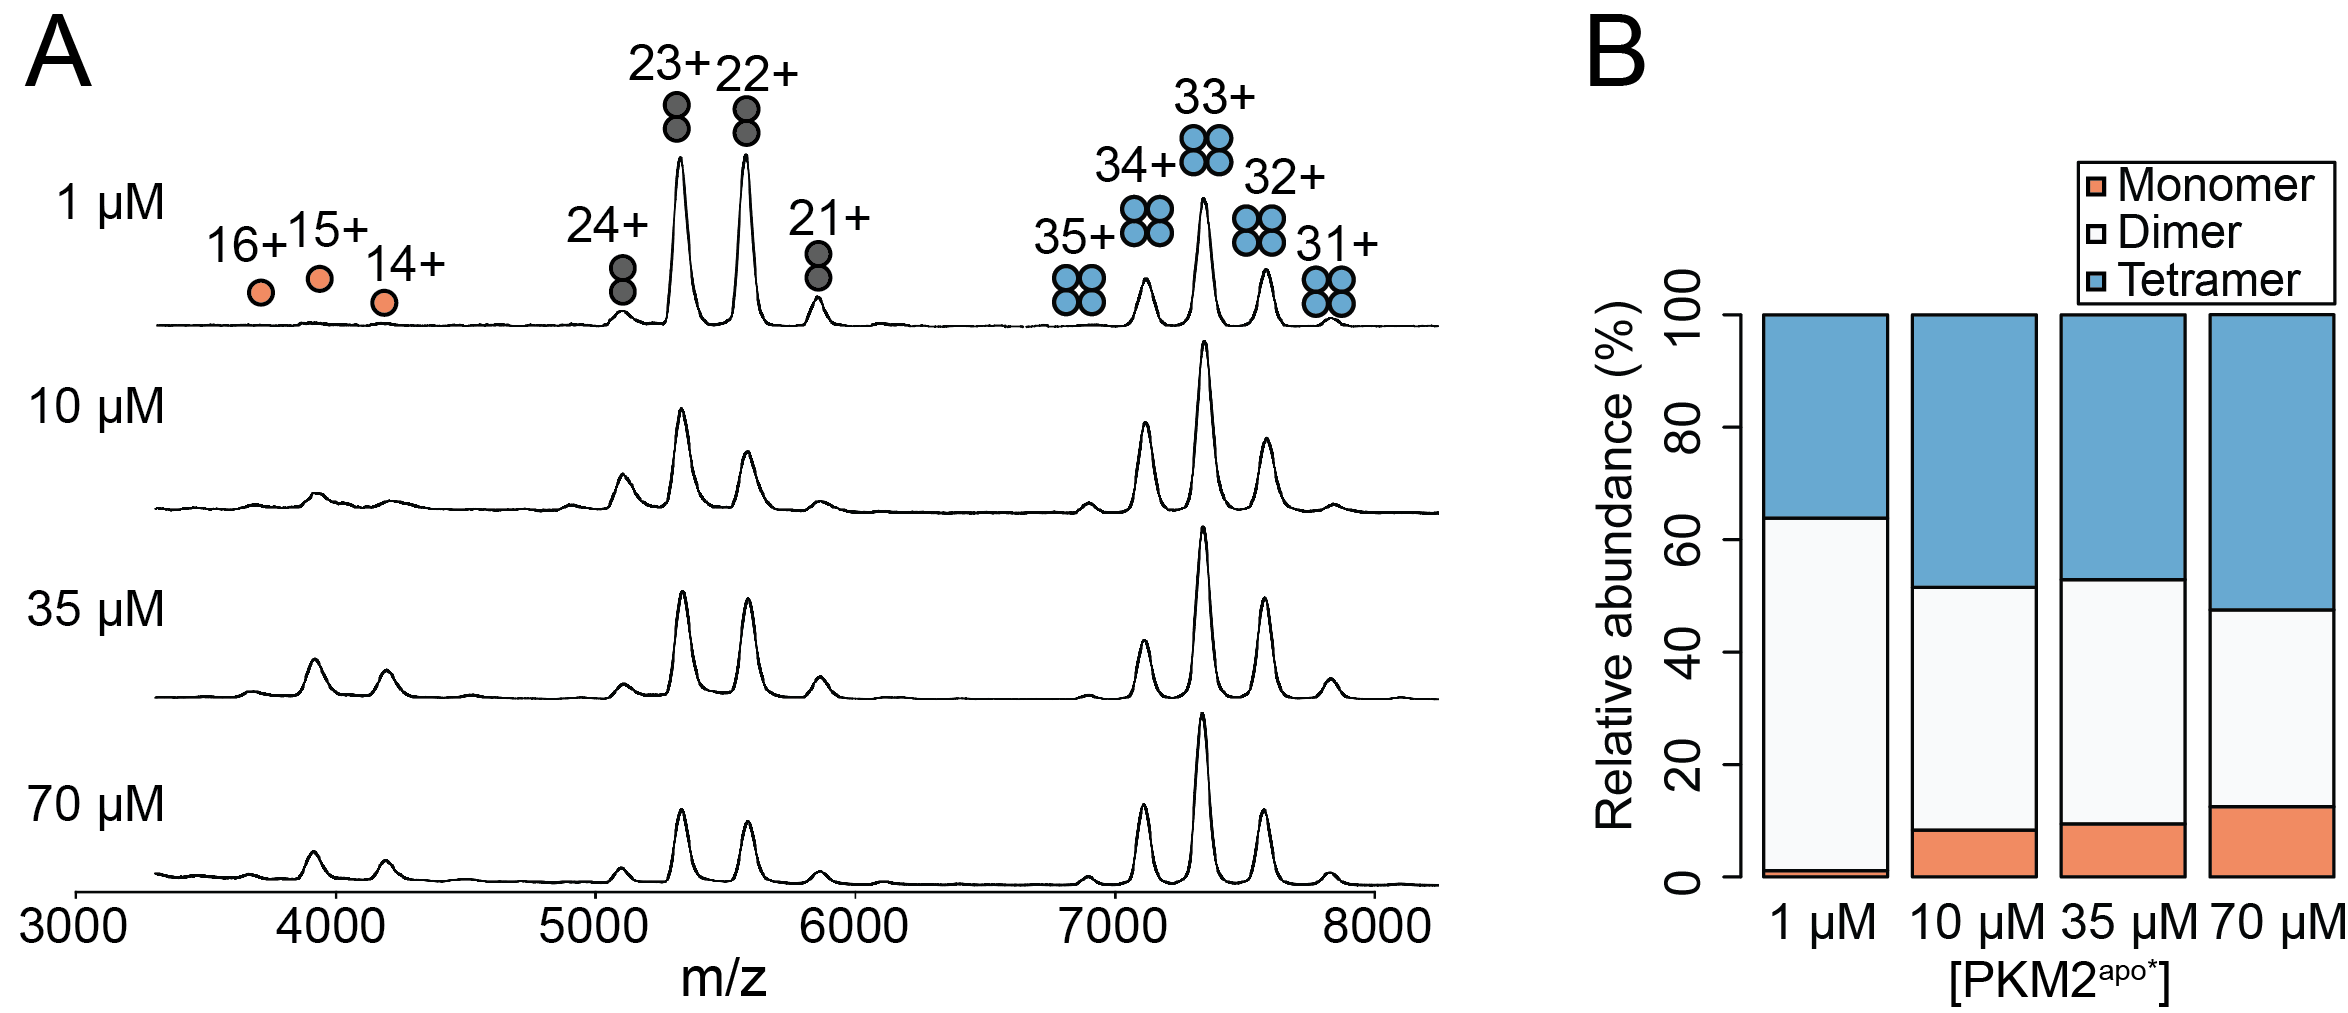
\includegraphics[scale=0.8]{ch5_fig1_pkm2conc.png}
\caption[The concentration-dependence of PKM2 oligomerisation.] {\textbf{The concentration-dependence of PKM2 oligomerisation.} \textbf{(A)} Nano-electrospray ionisation mass spectrometry was used to acquire native spectra of PKM2$^{apo \ast}$. The protein was sprayed from a 100 mM ammonium acetate solution containing a total PKM2 concentration of 1 $\mu$M, 10 $\mu$M, 35 $\mu$M and 70 $\mu$M. \textbf{(B)} The oligomeric state distribution was quantified for each of the concentration of PKM2 and presented as stacked bars showing the relative intensities of monomers (orange), dimers (white) and tetramers (blue).}
\label{fig:pkm2_conc}
\end{figure}
%
%
\clearpage


\subsection{PKM2 dimers form stably about the A-A' interface}
\label{subsec:aa_dimer_imms}

\subsubsection{PKM2 dimers might form two possible assembles about the A-A' and C-C' interfaces}
The inherent two-fold symmetry of PKM2 tetramers may give rise to one of two possible dimeric assemblies about the A-A' interface (the A-A' dimer) or about the C-C' interface (the C-C' dimer) (\textbf{Fig. \ref{fig:dimer_imms} A}). It was unclear whether the PKM2 dimers observed in the native spectra (\textbf{Fig. \ref{fig:pkm2_conc} A}) were of the A-A' or C-C' assembles, or a mixture of the two. PKM2 protomers have the same primary structure and hence, identical masses, and so it was not possible to mass-resolve the two possible species. Nevertheless, an inspection of the overall shape of \textit{in silico} models generated of the two dimeric assemblies showed a difference in shape between the two possible dimer species (the A-A' dimer is more globular than the elongated C-C' dimer assembly; \textbf{Fig. \ref{fig:dimer_imms} A}). As such, we hypothesised that the two dimer assemblies could be distinguished by their mobilities in the gas phase.

\subsubsection{\textit{In silico} calculations find that A-A' and C-C' dimers have distinct ion mobilities}
To this end, we used IM-MS to measure the experimental drift time of selectively activated PKM2 dimer charge states. The drift time of the ion in a defined buffer gas ($t_{D}$) is proportional to the rotationally-averaged collision cross section (CCS, $\Omega$), which can be interpreted as the shape adopted by a given molecular ion under particular gas phase conditions \cite{Jurneczko:2011aa}:
%
%
\begin{equation}
\Omega = \frac{ \sqrt{18 \pi }}{16} \frac{ze}{\sqrt{k_{B}T}} \left[ \frac{1}{m_{I}} + \frac{1}{m_{N}} \right]^{0.5} \frac{t_{D}E}{L} \frac{760}{P} \frac{T}{273.2} \frac{1}{N}
\end{equation}
%
%
where $e$ is the elementary charge, $E$ is the charge carried by the ion, $N$ is the number density, $L$ is the path length of the drift cell, $T$ is the temperature and $k_{B}$ is the Boltzmann constant.
%
%
\\\\
%
%
For comparison with experimental measurements, the CCS of the 23+ A-A' and C-C' dimers, the 15+ monomer and the 33+ tetramer ions were computed from short 10 ns molecular dynamics simulations of A-A' and C-C' dimer \textit{in silico} models (see Methods Section \ref{methods:vacuo_md}). The CCS was calculated from the representative clustered structures using a projection-approximation (PA) approach ($^{PA}CCS$), which has been used for many years to calculate rotationally-averaged CCS values for molecules \cite{Jurneczko:2011aa}. PA methods, however, fail to account for long-range interactions and all the physical details of the scattering process between the ion and the buffer gas \cite{Jurneczko:2011aa}. For a more explicit treatment of the scattering process in calculating the CCS, $^{PA}CCS$ was supplemented with additional CCS calculations using an elastic hard-sphere scattering (EHSS) approach ($^{EHSS}CCS_{He}$), in which the CCS is calculated by averaging the momentum transfer cross section which is related to the scattering angles between the incoming and departing gas atom trajectory \cite{Jurneczko:2011aa}. 

\subsubsection{A comparison between theoretical and experimental CCS measurements finds that dimeric PKM2 forms the A-A' assembly}
The experimentally determined collision cross section for the 15+ monomer ion ($^{DT}CCS_{He}$) was (34.\textcolor{red}{5} $\pm$ 9.9) $nm^2$, 3.3 \% larger than the theoretical $^{EHSS}CCS_{He}$ (\textbf{Fig. \ref{fig:dimer_imms} B}). Although the difference between the $^{EHSS}CCS_{He}$ and the experimental $^{DT}CCS_{He}$ was found to be significant (p-value < 0.001), a more pronounced structural compaction in gas-phase molecular dynamics simulations has been previously reported to manifest in smaller collision cross sections, relative to the experimental measurements \cite{Pacholarz:2017aa}. The theoretically determined $^{PA}CCS$ was found to further underestimate the experimental $^{DT}CCS_{He}$ by 10.1 \% [$^{PA}CCS$ = (31.00 $\pm$ 1.71) $nm^2$] (\textbf{Fig. \ref{fig:dimer_imms} B}), likely because the PA approach does not account for the effects of multiple ion-gas collisions, and hence for ions of masses greater than 2 kDa, this method will underestimate the CCS and is know to be of limited use for the study of larger biomolecules \cite{Jurneczko:2011aa}. 
%
%
\\\\
%
%
The experimentally measured $^{DT}CCS_{He}$ for the 33+ tetramer ion [(92.46 $\pm$ 2.57) $nm^2$] was in good agreement with the theoretically-determined CCS as determined using the EHSS-approach [$^{EHSS}CCS_{He}$ = (92.98 $\pm$ 3.41) $nm^2$] (\textbf{Fig. \ref{fig:dimer_imms} B}). Taken together, the agreement between theoretically and experimentally determined CCS values for PKM2 monomer and tetramer ions suggested that similar measurements of the dimer ion would have predictive power in elucidating the assembly of dimeric PKM2 in the gas phase.
%
%
\\\\
%
%
The C-C' dimer was found to have a theoretical CCS of [$^{EHSS}CCS_{He}$ = (61.08 $\pm$ 6.73) $nm^2$], 13 \% larger than the A-A' dimer [$^{EHSS}CCS_{He}$ = (53.20 $\pm$ 2.23) $nm^2$] (\textbf{Fig. \ref{fig:dimer_imms} B}), suggesting that the two possible dimer assemblies have distinct ion mobilities. Experimental CCS measurements of the 21+ dimer ion [$^{DT}CCS_{He}$ = (52.59 $\pm$ 9.37) $nm^2$] were in close agreement with the theoretically-determined CCS of the A-A' dimer (\textbf{Fig. \ref{fig:dimer_imms} B}). The close match between the theoretical CCS of the A-A' dimer and the experimentally-measured CCS of dimeric PKM2, suggested that PKM2 dimers form the A-A' assembly in the gas phase. 
%
%
%
%
%%% FIGURE
%
\begin{figure}[!ht]
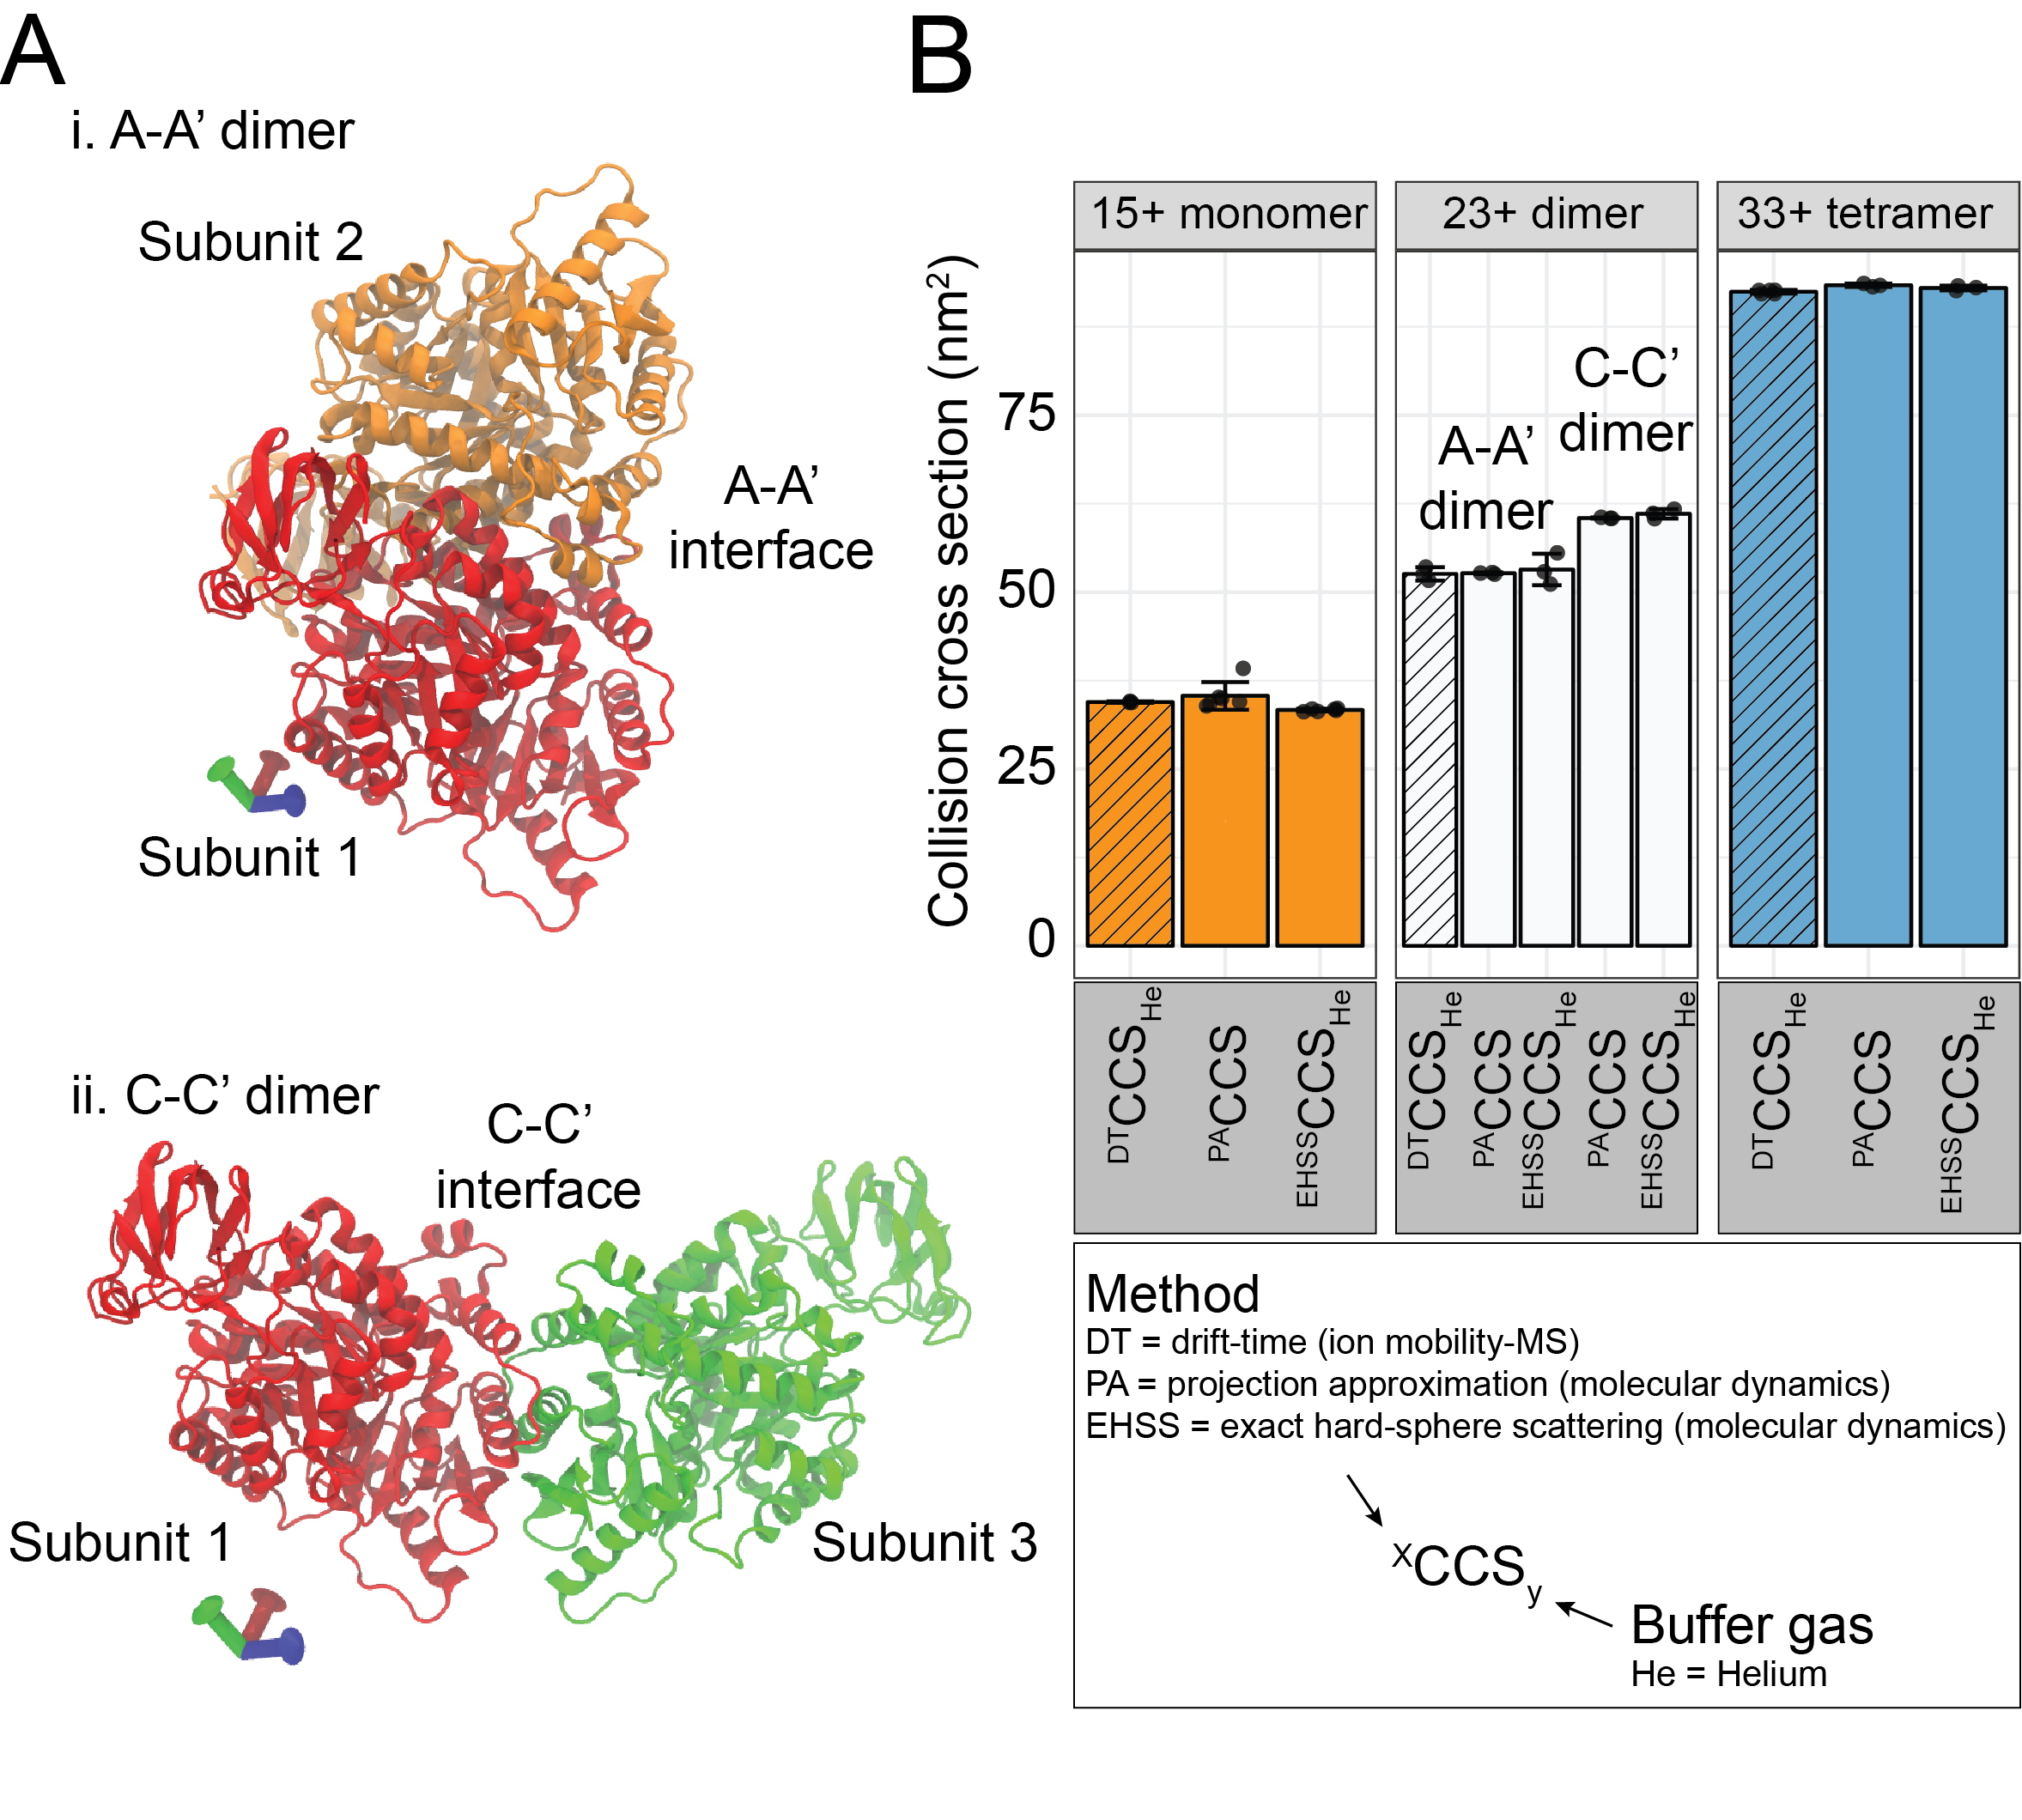
\includegraphics[scale=0.7]{ch5_fig4_dimer_imms.png}
\caption[Ion mobility measurements reveal that PKM2 dimers are stable about the A-A' interface.] {\textbf{Ion mobility measurements reveal that PKM2 dimers are stable about the A-A' interface.} \textbf{(A)} Structural models of [i] A-A' dimers and [ii] C-C' dimers, shown in cartoon representation. \textbf{(B)} The CCS of the 15+ monomeric (orange), 23+ dimeric (white) and 33+ tetrameric (blue) $PKM2^{apo \ast}$ calculated experimentally by IM-MS (shaded bars) and from MD simulations of the respective ions using the Projection Approximation ($^{PA}CCS$) and Exact Hard-Sphere Scattering ($^{EHSS}CCS_{He}$) approaches.}
\label{fig:dimer_imms}
\end{figure}
%
%
\clearpage

\subsection{FBP induces PKM2 tetramerisation}
\label{subsec:fbp_tetramerisation}
Consistent with previous studies \cite{Yacovan:2012aa,Jiang:2010aa,Dombrauckas:2005aa,Chaneton:2012aa}, a characterisation of enzyme kinetics of PKM2 in Chapter \ref{chapter:enzyme_kinetics} showed that the binding of FBP increases the effective substrate affinity of PKM2 for phosphoenolpyruvate. To explore whether this functional effect of activator binding was accompanied by an induced change in the oligomeric state, we acquired native spectra of PKM2 titrated with FBP. FBP addition was found to increase the relative abundance of tetrameric charged-state species in a dose-dependent manner (\textbf{\ref{fig:pkm2_fbp_MS} A} and \textbf{B}).  Additionally, an apparent m/\textit{z} shift in the tetrameric peaks and a qualitative change to the overall charged-state envelope was observed (\textbf{\ref{fig:pkm2_fbp_MS} C}). The m/\textit{z} shift was expected to result from the binding of at least three molecules of FBP to each PKM2 tetrameric species, given that preparation of protein had been previously characterised as containing $\simeq$ 23 \% of the binding sites pre-occupied with co-purified FBP (Section \ref{subsec:fbp_binding_pkm2}).
%
%
%
%
%%% FIGURE
%
\begin{figure}[!ht]
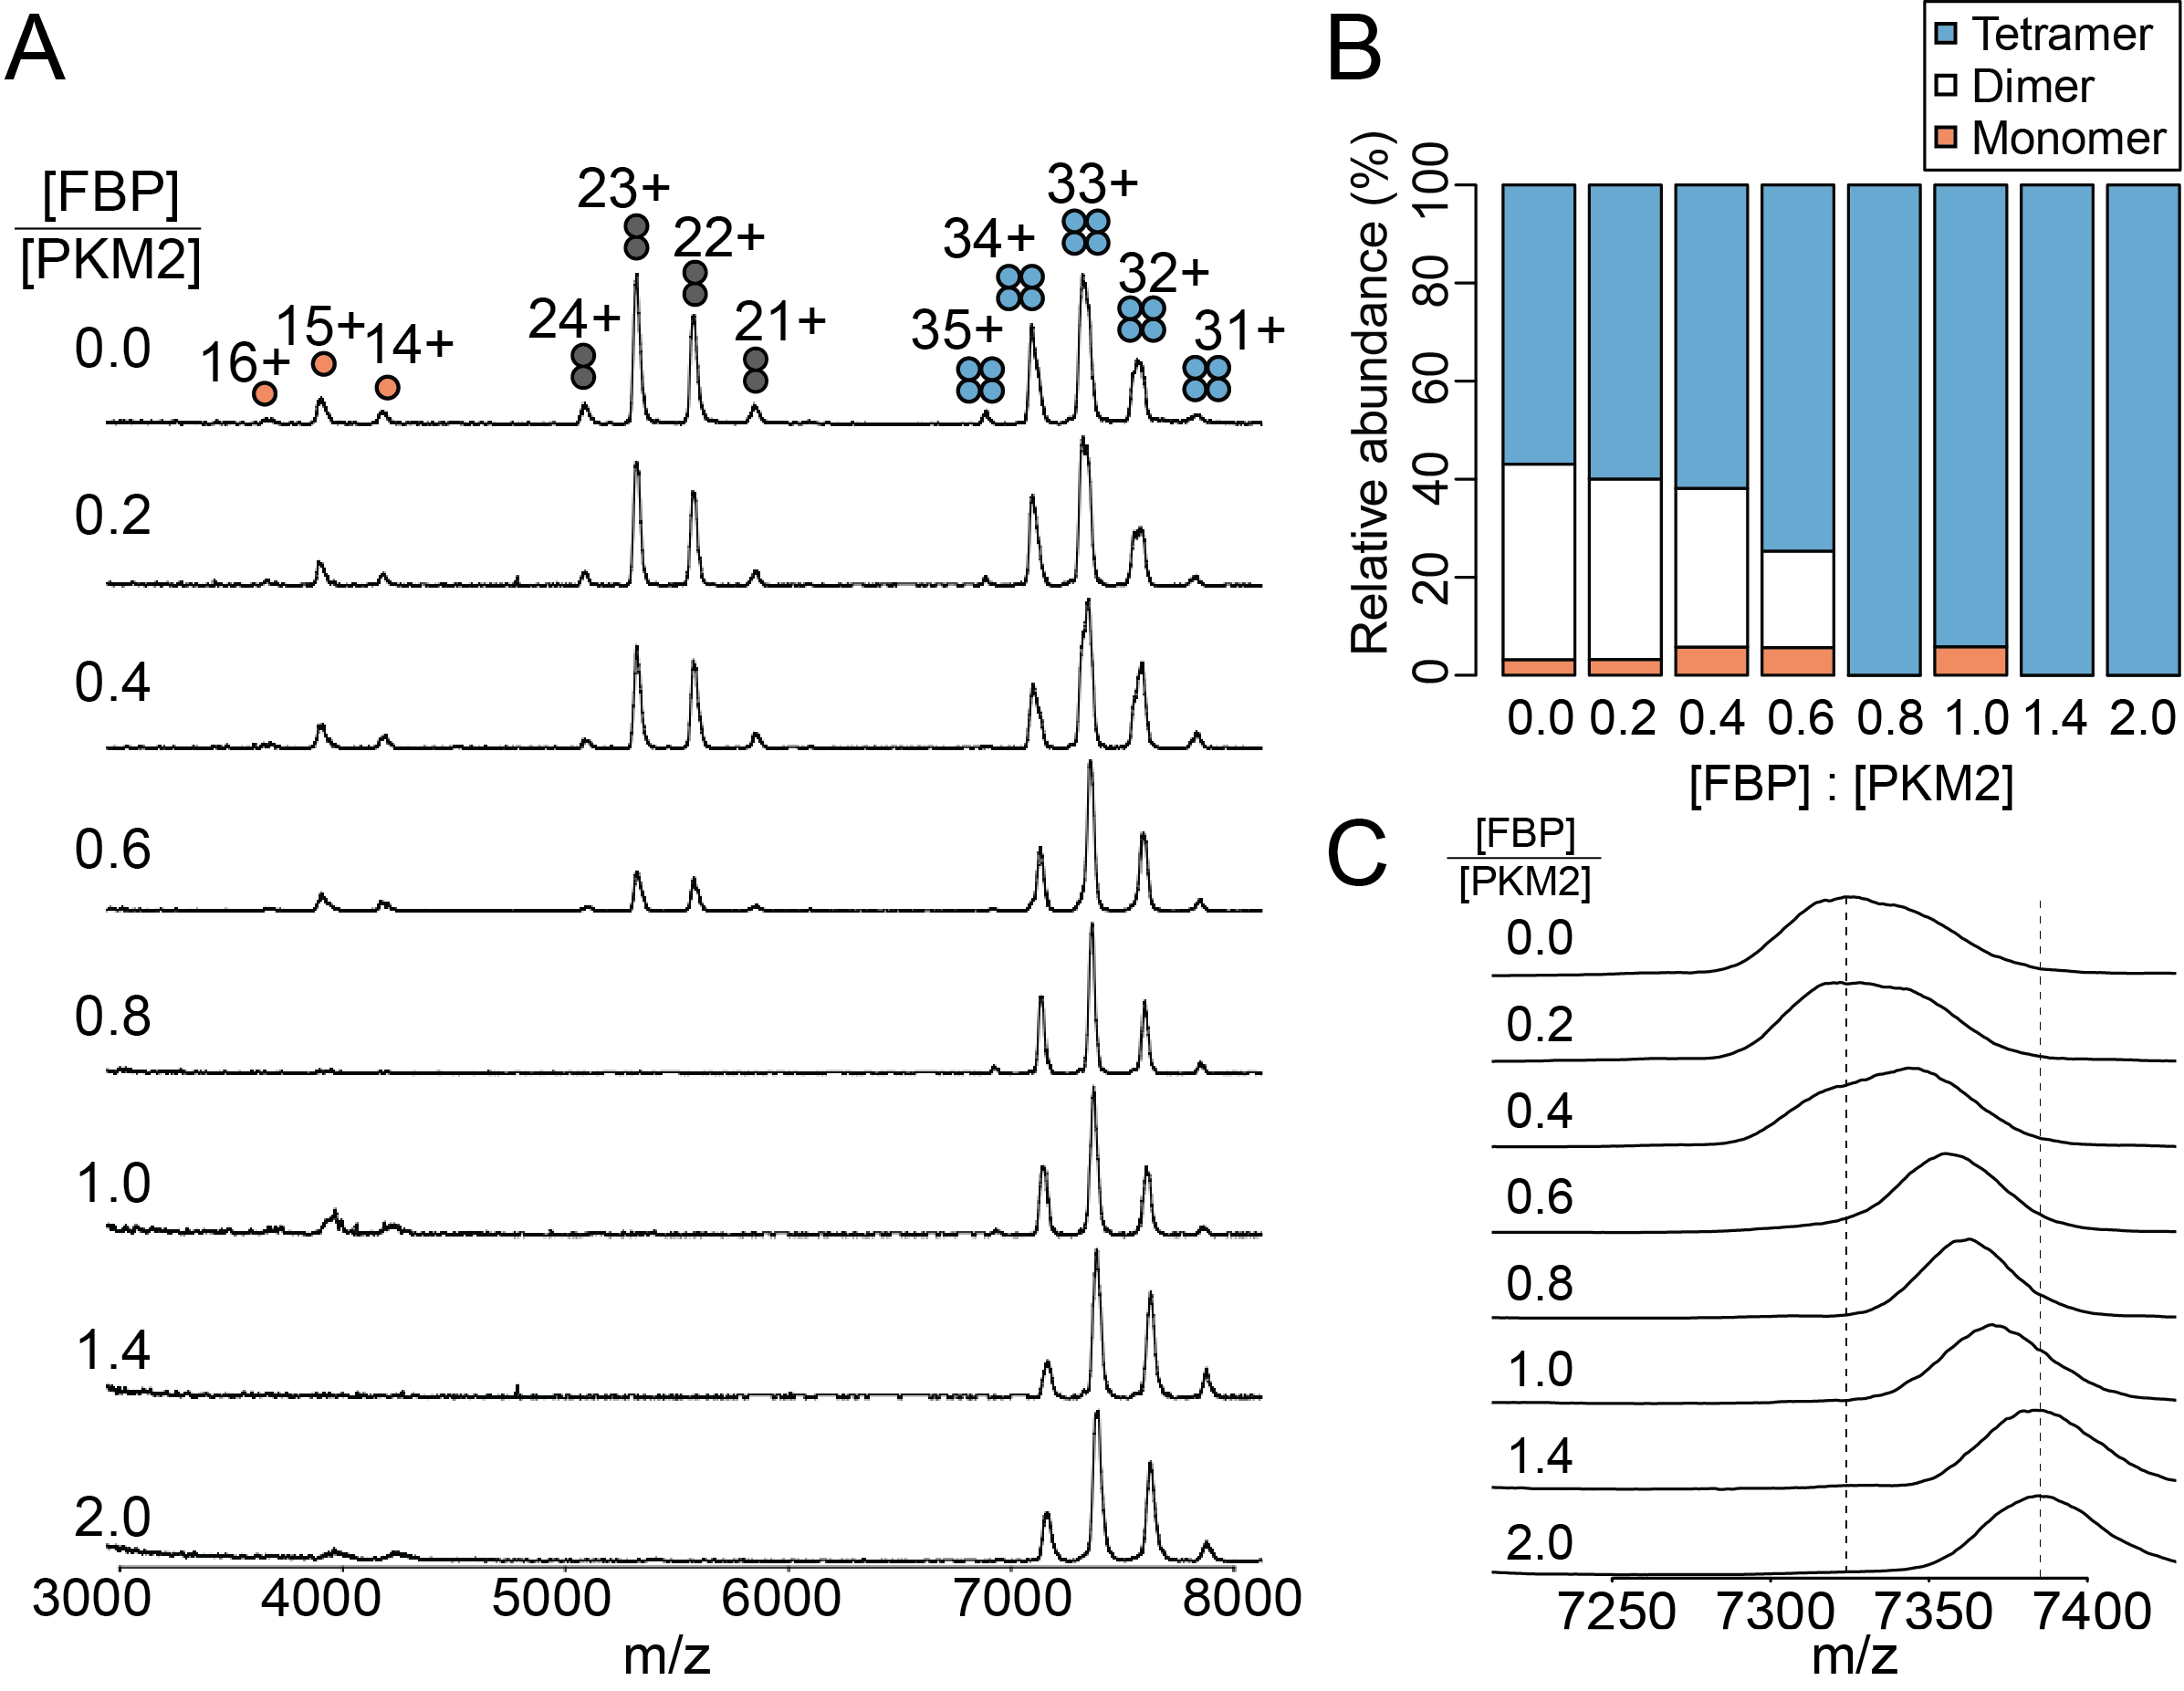
\includegraphics[scale=0.7]{ch5_fig2_fbp_MS.png}
\caption[FBP addition induces a dose-dependent tetramerisation of PKM2.] {\textbf{FBP addition induces a dose-dependent tetramerisation of PKM2.} \textbf{(A)} Native spectra were acquired for PKM2 titrated with FBP. The ratio of protein-to-ligand is indicated. \textbf{(B)} The relative intensities of oligomeric states was determined for each ratio-metric mixture of FBP-PKM2. \textbf{(C)} Native spectra of the 33+ tetrameric charge state species for each stoichiometric mixture of FBP-PKM2.}
\label{fig:pkm2_fbp_MS}
\end{figure}
%
%
\clearpage


\subsection{PKM2$^{Apo \ast}$ tetramers are formed from a mixture of apo and holo protein}
In order to resolve the apparent mass shift of tetrameric PKM2 upon FBP addition, spectra of PKM2 were acquired under high cone-voltage conditions in order to remove salt adducts during the ionisation process, which would otherwise add to the overall weight of analyte ions. Mass-deconvolution of the subsequent spectra (see Methods Section \ref{methods:mass_deconv_ms}) could thus be compared to the theoretical mass of the PKM2 from its primary sequence. 
%
%
\\\\
%
%
The mass-deconvolved spectrum of FBP-saturated PKM2 ($PKM2^{FBP}$) revealed a single mass peak at 234.190 kDa (\textbf{Fig. \ref{fig:pkm2_mass_spectrum}}) corresponding to the theoretical mass of tetrameric PKM2 bound to four molecules of FBP (234.273 kDa). In contrast, tetrameric PKM2 in the absence of any added FBP ($PKM2^{apo \ast}$), consisted of five separate peaks (\textbf{Fig. \ref{fig:pkm2_mass_spectrum}} and Table \ref{table:native_masses}). The difference in mass between the different $PKM2^{apo \ast}$ mass peaks were approximately equivalent to the mass equivalents of a single molecule of FBP (340 Da), suggesting that the peaks reflected tetrameric PKM2 species bound to 0, 1, 2, 3 and 4 molecules of FBP (\textbf{Fig. \ref{fig:pkm2_mass_spectrum}}). The intensities of the five mass peaks of PKM2 in the absence of added FBP, reaffirmed the finding that considerable molar amounts of FBP are retained during the purification of PKM2 (Section \ref{subsec:fbp_binding_pkm2}). Additionally, these results show that FBP binding is not required for PKM2 tetramer formation. Moreover, the relative apex-intensities of the five mass peaks of $PKM2^{apo \ast}$ may provide information on the degree of cooperativity associated with FBP binding. For an infinitely cooperative system, where the concentration of ligand is limiting, one would expect appreciable quantities of only the \textit{apo} and \textit{holo} species. The distribution of peaks with an approximate ratio of 5:2:2:2:1, however, suggests that FBP binding is weakly cooperative.

%%%%%%%%%%%%%%%%
%% 	Mass tables		    %%
%%%%%%%%%%%%%%%%

\begin{table}[!ht]
\centering
\caption{Theoretically-determined masses of PKM2 and FBP}
\begin{tabular}{@{}ll@{}}
\toprule
Molecule                                  & Mass (Da)                      \\ \midrule
Monomeric PKM2                            & 58218.16                       \\
Tetrameric PKM2                           & 232872.60                      \\
D-fructose-1,6-bisphosphate               & 350.0                          \\
Tetrameric PKM2 + 1 FBP					& 233222.6						   \\
Tetrameric PKM2 + 2 FBP					& 233572.6						   \\
Tetrameric PKM2 + 3 FBP					& 233922.6						   \\
Tetrameric PKM2 + 4 FBP					& 234272.6						   \\ 
\bottomrule
\end{tabular}
\label{table:theoretical_masses}
\end{table}
%
%
\begin{table}[!ht]
\centering
\caption{Maximum entropy mass estimation of tetrameric PKM2 from nESI-MS m/z spectra under native-like and high cone-voltage ionisation conditions.}
\begin{tabular}{@{}llll@{}}
\toprule
System                                                                         & Conditions   & \begin{tabular}[c]{@{}l@{}}Number of tetramer\\ peaks\end{tabular} & Mass (Da)                      \\ \midrule
10 $\mu M$ PKM2                                                                & High voltage & 4                                                                  & 232880, 233220, 233580, 233930, 234290 \\ 
+ 10 $\mu M$ FBP                                                               & Native-like  & 1                                                                  & 235030                         \\ 
+ 10 $\mu M$ FBP                                                               & High voltage & 1                                                                  & 234190                         \\ 
\bottomrule
\end{tabular}
\label{table:native_masses}
\end{table}
%
%
%
%
%%% FIGURE
%
\begin{figure}[!ht]
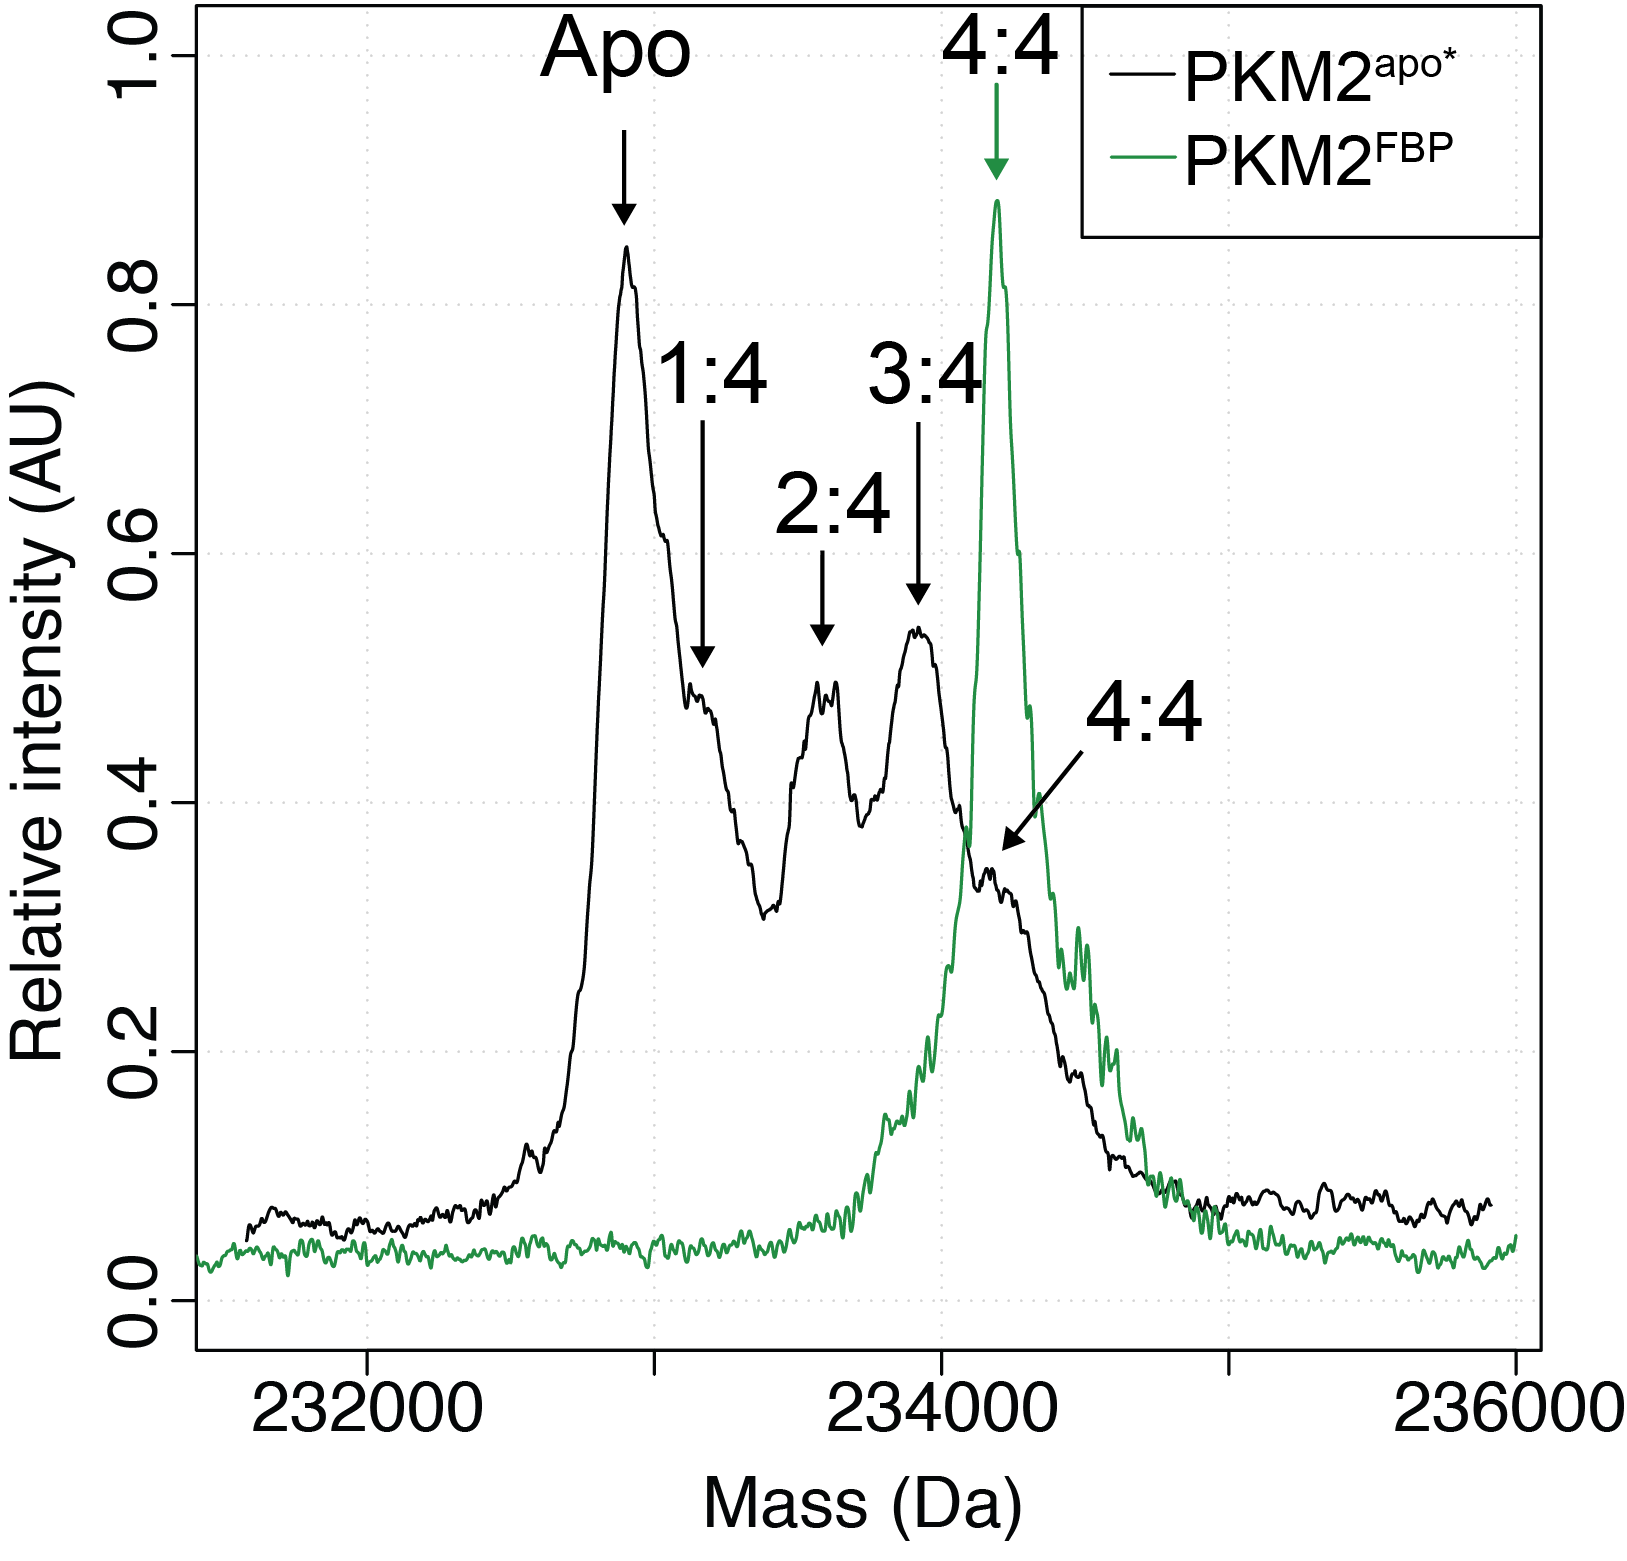
\includegraphics[scale=0.7]{ch5_fig3_fbp_mass_deconv.png}
\caption[The mass-deconvolved spectrum of $PKM2^{apo \ast}$ reveals a mixture of \textit{apo} and \textit{holo} species.] {\textbf{The mass-deconvolved spectrum of $PKM2^{apo \ast}$ reveals a mixture of \textit{apo} and \textit{holo} species.} Mass-deconvolved spectra were calculated from spectra of $PKM2^{apo}$ and $PKM2^{FBP}$. Normalised mass spectra of  $PKM2^{apo \ast}$ (black) and $PKM2^{FBP}$ (green) are shown. Peaks are annotated with the corresponding FBP-PKM2 stoichiometric species, as determined from the exact mass of the measurement.}
\label{fig:pkm2_mass_spectrum}
\end{figure}
%
%
\clearpage


\subsection{FBP binding induces subtle changes to the shape of tetrameric PKM2}
\label{subsec:fbp_ccsd}
Previous studies have suggested that allosteric ligands induce inter-domain conformational changes within the PKM2 tetramer \cite{Dombrauckas:2005aa,Gehrig:2017aa,Morgan:2013aa,Yan:2016aa} and other pyruvate kinase homologues \cite{Donovan:2016aa,Morgan:2010aa,Naithani:2015aa,Zhong:2017aa}. Therefore, we investigated the possibility that FBP binding induced conformational changes that could be detected by an altered mobility in the gas phase.
%
%
\\\\
%
%
To this end, IM-MS measurements of PKM2 were acquired in the absence and in the presence of saturating amounts of FBP, from which a global CCS was calculated for each tetramer (see Methods Section \ref{methods:imms_ccs}). We found that differences in the $^{DT}CCS_{He}$ distribution, which reflects the conformational heterogeneity of proteins, suggested that FBP caused subtle conformational changes in the tetramer (\textbf{Fig. \ref{fig:pkm2_fbp_ccsd}}). The negative difference in the $^{DT}CCS_{He}$ distribution between PKM2$^{apo \ast}$ and PKM2$^{FBP}$ at $^{DT}CCS_{He} > 10000$ suggested that FBP binding marginally reduces the compaction of the tetramer.
%
%
%
%
%%% FIGURE
%
\begin{figure}[!ht]
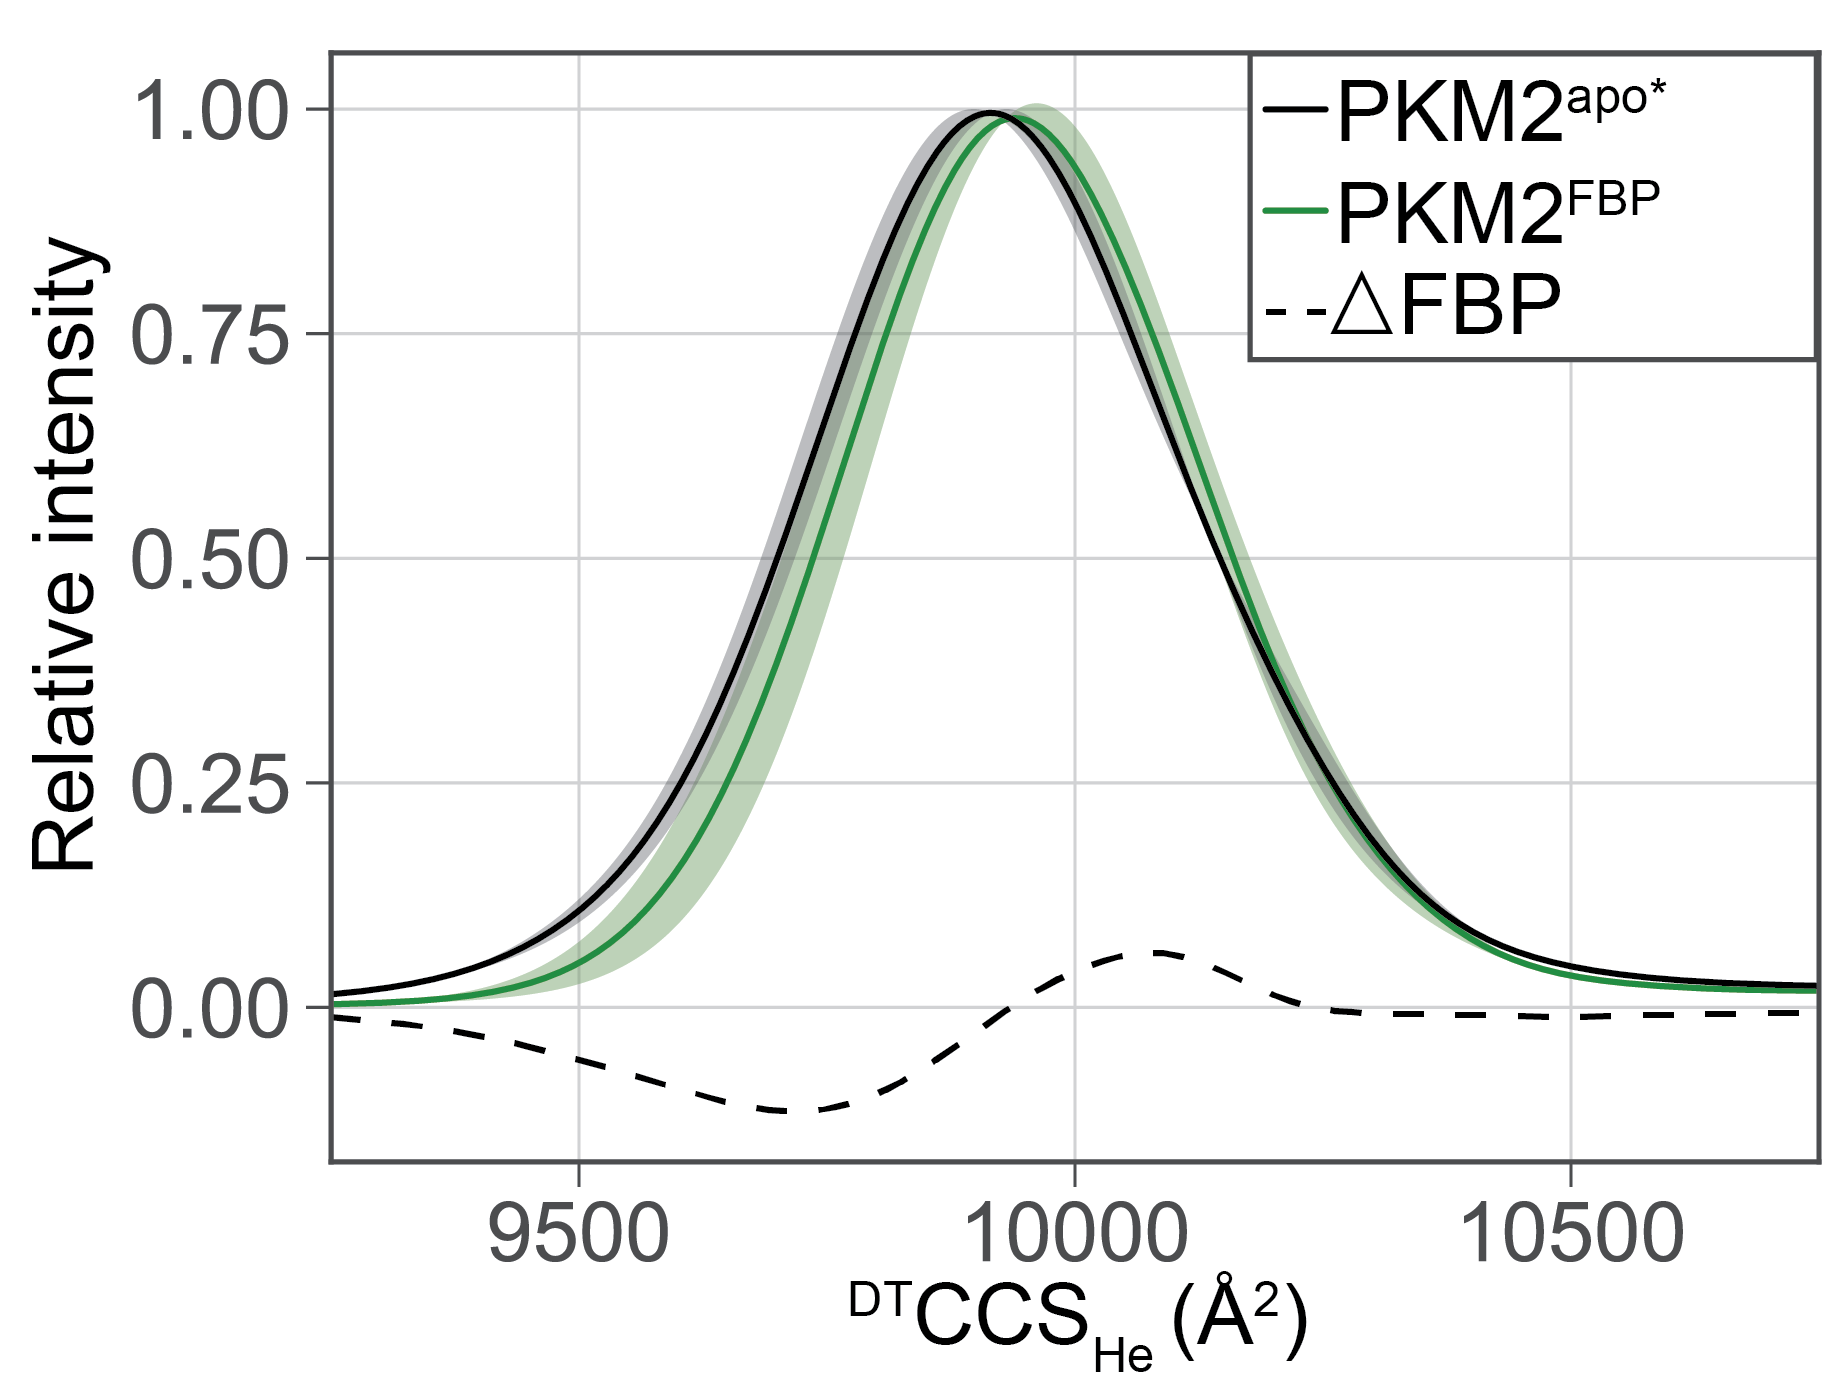
\includegraphics[scale=0.6]{ch5_fig7_fbp_global_ccs.png}
\caption[FBP binding changes the global collision cross section of PKM2 tetramers.] {\textbf{FBP binding changes the global collision cross section of PKM2 tetramers.} $^{DT}CCS_{He}$ distribution of PKM2$^{apo \ast}$ and PKM2$^{FBP}$ calculated from analyses of arrival time distribution measurements of PKM2 tetramer peaks (see Methods Section \ref{methods:imms_ccs}). Average calculated values are shown in solid lines and the standard deviations are shown as shaded ribbons. The difference spectrum between PKM2$^{apo \ast}$ and PKM2$^{FBP}$ is shown as a dashed line.}
\label{fig:pkm2_fbp_ccsd}
\end{figure}

\clearpage

\section{Inhibitory amino acids have distinct effects on tetramerisation depending on whether FBP is bound}
Measurements of the steady-state kinetics of PKM2 in Chapter \ref{chapter:enzyme_kinetics} found that while FBP addition promoted high substrate affinity, simultaneous addition of phenylalanine (Phe) and FBP prevented FBP from exerting its maximally activating allosteric effect by reducing the $k_{cat}$. nESI-MS experiments supported the hypothesis that FBP activation involves tetramerisation of PKM2, linking activation to the oligomeric state. Competing views of amino acid inhibition of PKM2 debate the effects of Phe and Ala binding on PKM2 oligomerisation \cite{Hofmann:1975aa,Yuan:2018aa,Morgan:2013aa}. We therefore set out to determine the effects of amino acids on the oligomeric state of PKM2, and to explore whether Phe impedes FBP-induced activation of PKM2 by affecting changes to the oligomeric state of the protein.


\subsection{Phe addition does not disrupt FBP-induced PKM2 tetramerisation}
\label{subsec:fbp_phe_nativems}
Addition either Phe to PKM2 at a protein-to-ligand ratio of 30:1, resulted in an increase in the relative abundance of dimeric PKM2 charge state species (\textbf{Fig. \ref{fig:aa_nms} A} and \textbf{B}), suggesting that Phe addition \textit{per se} favoured the dimeric form of PKM2. The perference of Phe for dimerisation is in agreement with previous solution-phase analytical ultracentrifugation studies \cite{Hofmann:1975aa,Feliu:1976aa}. Broadening of the dimeric and tetrameric charge state peaks was observed, likely due to additional salt molecules binding to the protein upon addition of high concentrations of the ligand (\textbf{Fig. \ref{fig:aa_nms} A} and \textbf{B}). The apparent effects of Phe addition in promoting the dimeric state of PKM2, while significant in its magnitude, may have been underestimated due to the stoichiometry of binding. Considering the measured binding affinities of both ligands, calculated estimates of the fraction of 10 $\mu$M PKM2 bound upon addition of 300 $\mu$M Phe is 0.68, leaving a considerable fraction of the unbound protein. Attempts at measuring native m/z spectra of PKM2 at higher ligand concentrations were unsuccessful due to the unacceptably high salt content of the protein-ligand mixture. 
%
%
\\\\
%
%
Next, native spectra of PKM2 were acquired following pre-incubation with saturating concentrations of FBP. As before (Section \ref{subsec:fbp_tetramerisation}), FBP addition resulted in PKM2 tetramerisation (\textbf{Fig. \ref{fig:phe_fbp_native_spectra} A} and \textbf{B}). Addition of Phe subsequent to pre-incubation with FBP did not perturb the tetrameric state of PKM2, while FBP binding to PKM2 pre-incubated with Phe resulted in protein tetramerisation, indicating that the dominant effect of FBP on PKM2 tetramerisation was not effected by the order of ligand addition (\textbf{Fig. \ref{fig:phe_fbp_native_spectra} A} and \textbf{B}).
%
%
%
%
%%% FIGURE
%
\begin{figure}[!ht]
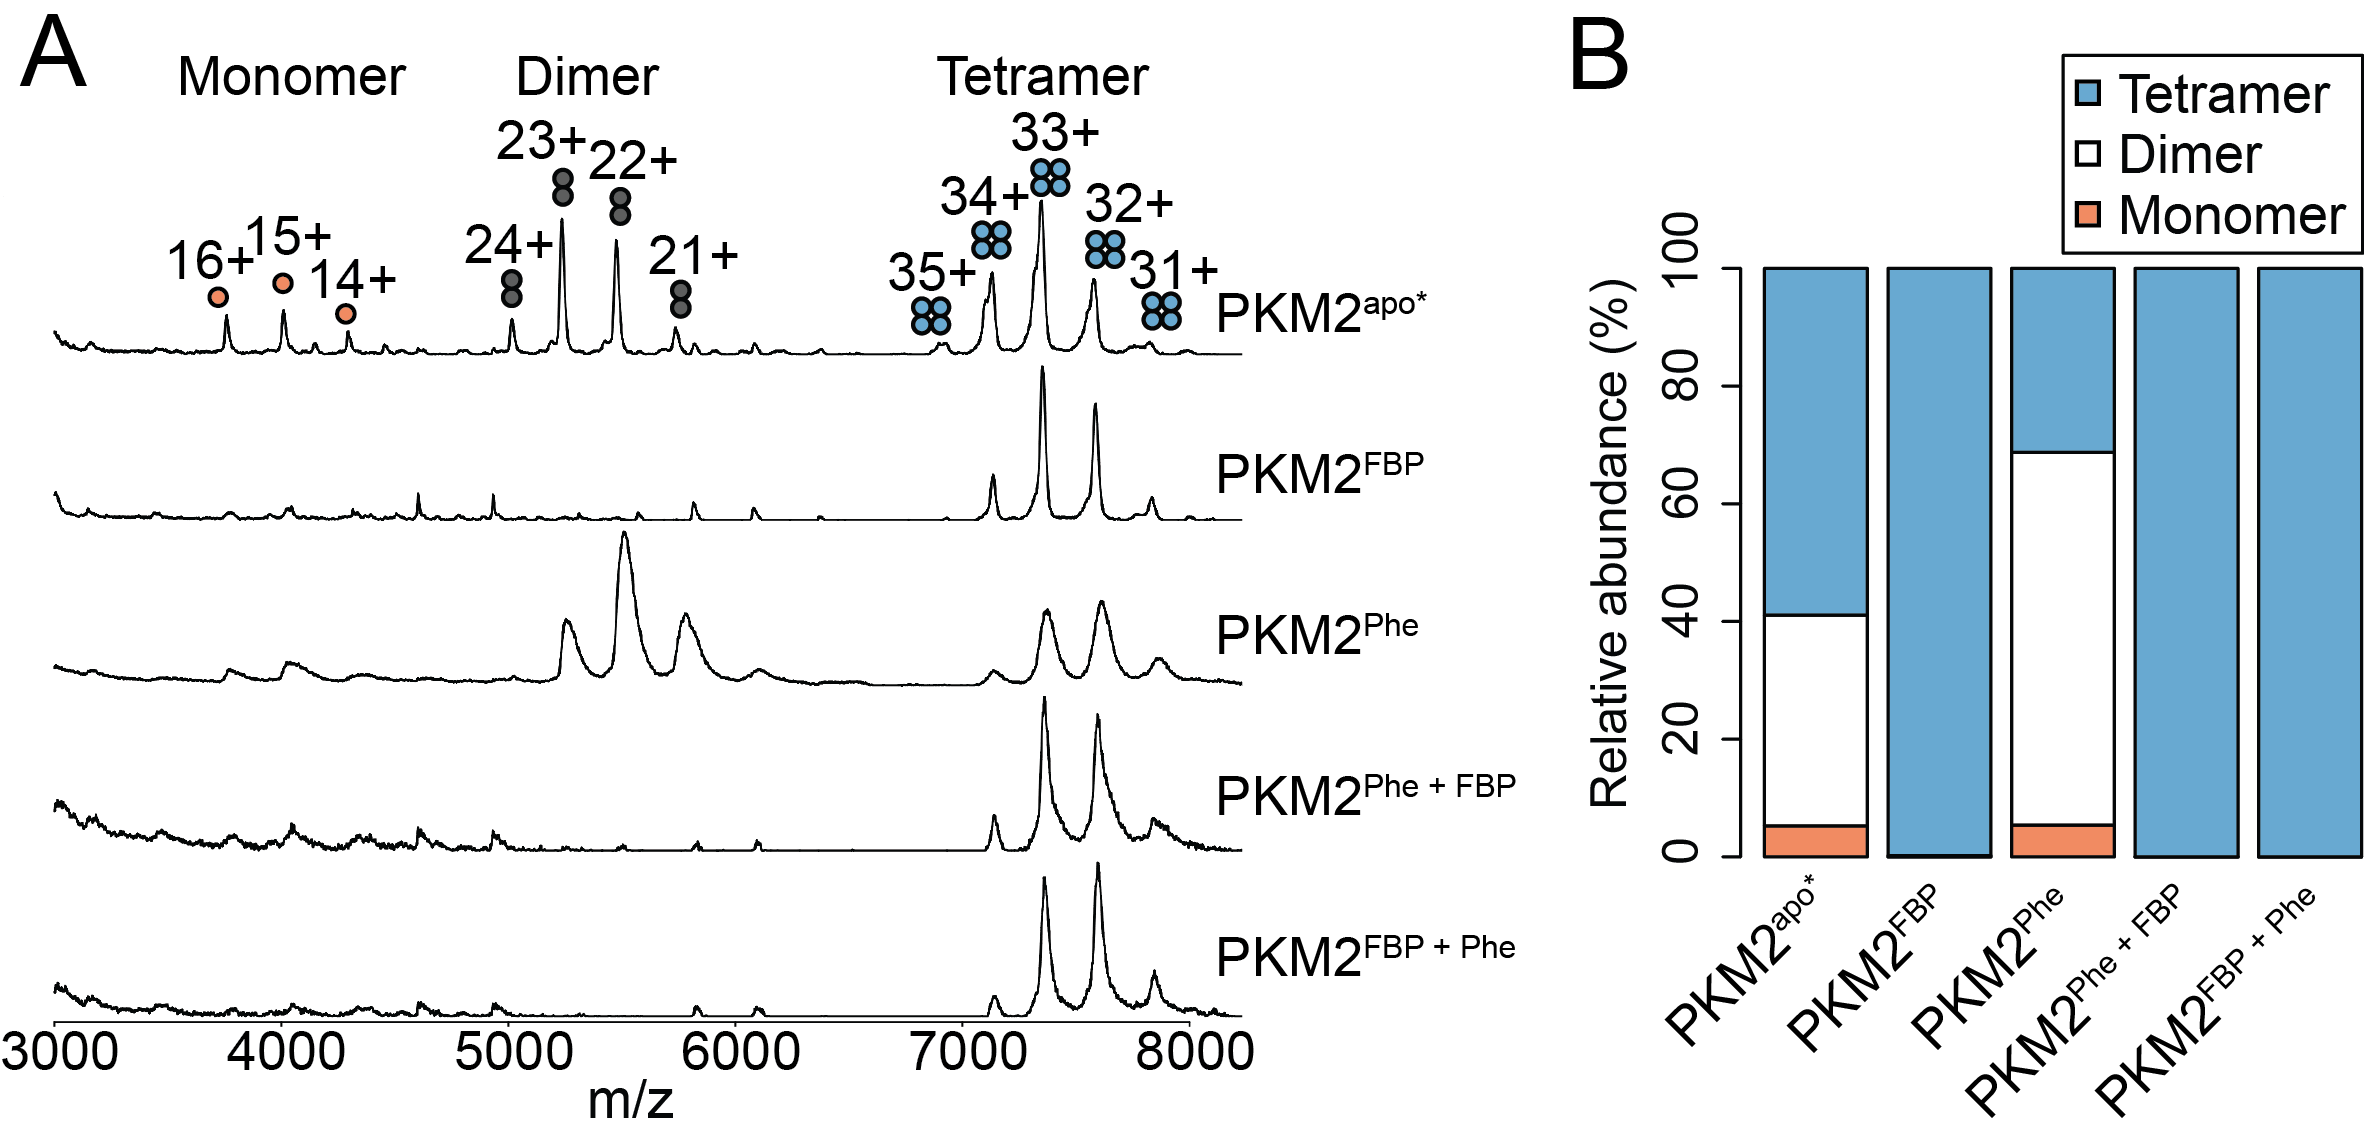
\includegraphics[scale=0.7]{ch5_fig9_fbp_phe_enms.png}
\caption[Phe binding does not disrupt FBP-induced PKM2 tetramerisation.] {\textbf{Phe binding does not disrupt FBP-induced PKM2 tetramerisation.} \textbf{(A)} Native spectra of 10 $\mu$M $PKM2^{apo \ast}$ and in the presence of 10 $\mu$M FBP ($PKM2^{FBP}$), 300 $\mu$M Phe $PKM2^{Phe}$, 300 $\mu$M Phe followed by addition of 10 $\mu$M FBP $PKM2^{Phe+FBP}$ and 10 $\mu$M FBP followed by addition of 300 $\mu$M Phe $PKM2^{FBP+Phe}$. Relative oligomeric state abundances were calculated and are shown in \textbf{(B)}. }
\label{fig:phe_fbp_native_spectra}
\end{figure}
%
%
\clearpage



\subsection{Phe and FBP synergistically promote PKM2 tetramerisation}
\label{subsec:phe_fbp_synergistic_tet}
It appeared from from the preceding native spectra of PKM2, that Phe had a neutral effect on the oligomeric state of FBP-bound PKM2 and that their binding was simply a passenger to FBP-induced tetramerisation. This hypothesis was found not to hold in the context of sub-stoichiometric FBP addition, where the subsequent addition of either Phe was found to act synergistically with FBP to promote PKM2 tetramerisation with slow kinetics [$k_{tet}$ = (812.5 $\pm$ 284.6) $s^{-1}$] (\textbf{Fig. \ref{fig:phe_fbp_time}}). Conversely, the addition of equivalent half-stoichiometric amount of FBP in the absence of Phe, were unable to fully convert PKM2 monomers and dimers into tetramers (\textbf{Fig. \ref{fig:phe_fbp_time}}). The propensity for Phe to enhance FBP-induced tetramerisation implied a functional synergism between the activator and either amino acid inhibitors, favouring tetramer formation despite to apparent opposing effects of these ligands, individually, both on enzyme activity and oligomerisation.
%
%
%
%
%%% FIGURE
%
\begin{figure}[!ht]
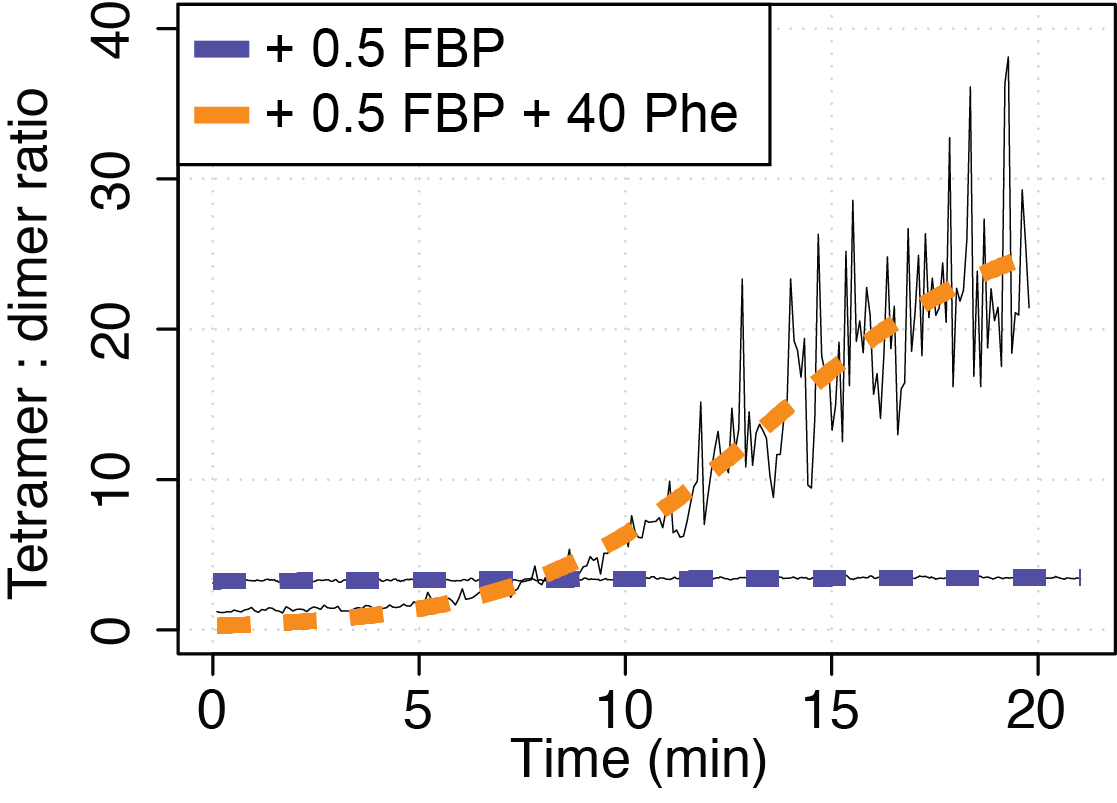
\includegraphics[scale=0.8]{ch5_fig10_fbp_phe_tet_time.png}
\caption[FBP and Phe synergistically promote PKM2 tetramerisation.] {\textbf{FBP and Phe synergistically promote PKM2 tetramerisation.} The time-resolved ratio of tetramer-to-dimer charge state intensities of 10 $\mu$M PKM2 following pre-incubation with either (i) 5 $\mu$M FBP, or (ii) 5 $\mu$M and 400 $\mu$M Phe. Time-resolved intensities are fit to a two-state sigmoidal model.}
\label{fig:phe_fbp_time}
\end{figure}
%
%
\clearpage

\subsection{Analytical evidence for simultaneous binding of FBP and Phe to PKM2}
The failure of Phe addition to destabilise FBP-bound PKM2 tetramers suggested a dominant effect of FBP on the oligomeric state of the protein. Moreover, it was predicted that the simultaneous addition of Phe and FBP to PKM2 would result in doubly-liganded PKM2, given the the finding from ligand binding studies that the binding affinity of Phe was unaffected by FBP binding, and \textit{vice versa}. Nevertheless, to address the possibility that under ionising conditions into the gas phase Phe does not bind to PKM2$^{FBP}$, we sought analytical evidence for simultaneous binding of Phe and FBP to PKM2.
%
%
\\\\
%
%
Evidence for concurrent Phe and FBP binding to PKM2 was provided by the m/\textit{z} shift produced by ligand addition to PKM2. Close inspection of the +33 tetramer charge state found that the PKM2$^{apo \ast}$ spectrum contained a doublet of tetramer peaks: the left portion of the peak was the fully-apo protein and the right portion resulted from ions of 1, 2, 3 and 4 FBP molecules bound to PKM2 tetramers (\textbf{Fig. \ref{fig:fbp_phe_binding_ms} A}). Addition of saturating amounts of FBP resulted in a small m/z shift towards higher CSD values (\textbf{Fig. \ref{fig:fbp_phe_binding_ms} A}). A further shift of the PKM2$^{FBP}$ 33+ peak was observed upon addition of Phe to FBP-bound PKM2 (\textbf{Fig. \ref{fig:fbp_phe_binding_ms} A}).
%
%
\\\\
%
%
The shift towards lower charge-states upon addition of Phe was found to be reversible when the cone voltage (CV) in the electrospray ionisation source was increased from 10 V to 100 V. Increasing the CV had the observed effect of reducing the negative charge of the PKM2$^{FBP + Phe}$ peaks and converting them to align with the PKM2$^{FBP}$ (\textbf{Fig. \ref{fig:fbp_phe_binding_ms} A}). This was achieved by displacing Phe molecules bound to PKM2$^{FBP}$. Conversely, increasing the CV of the ESI source did not convert the +33 PKM2$^{FBP}$ ion to the 'apo-like', suggesting that the high FBP-PKM2 binding affinity stabilised the interaction from dissociation even at high ionisation energies.
%
%
%
%
%%% FIGURE
%
\begin{figure}[!ht]
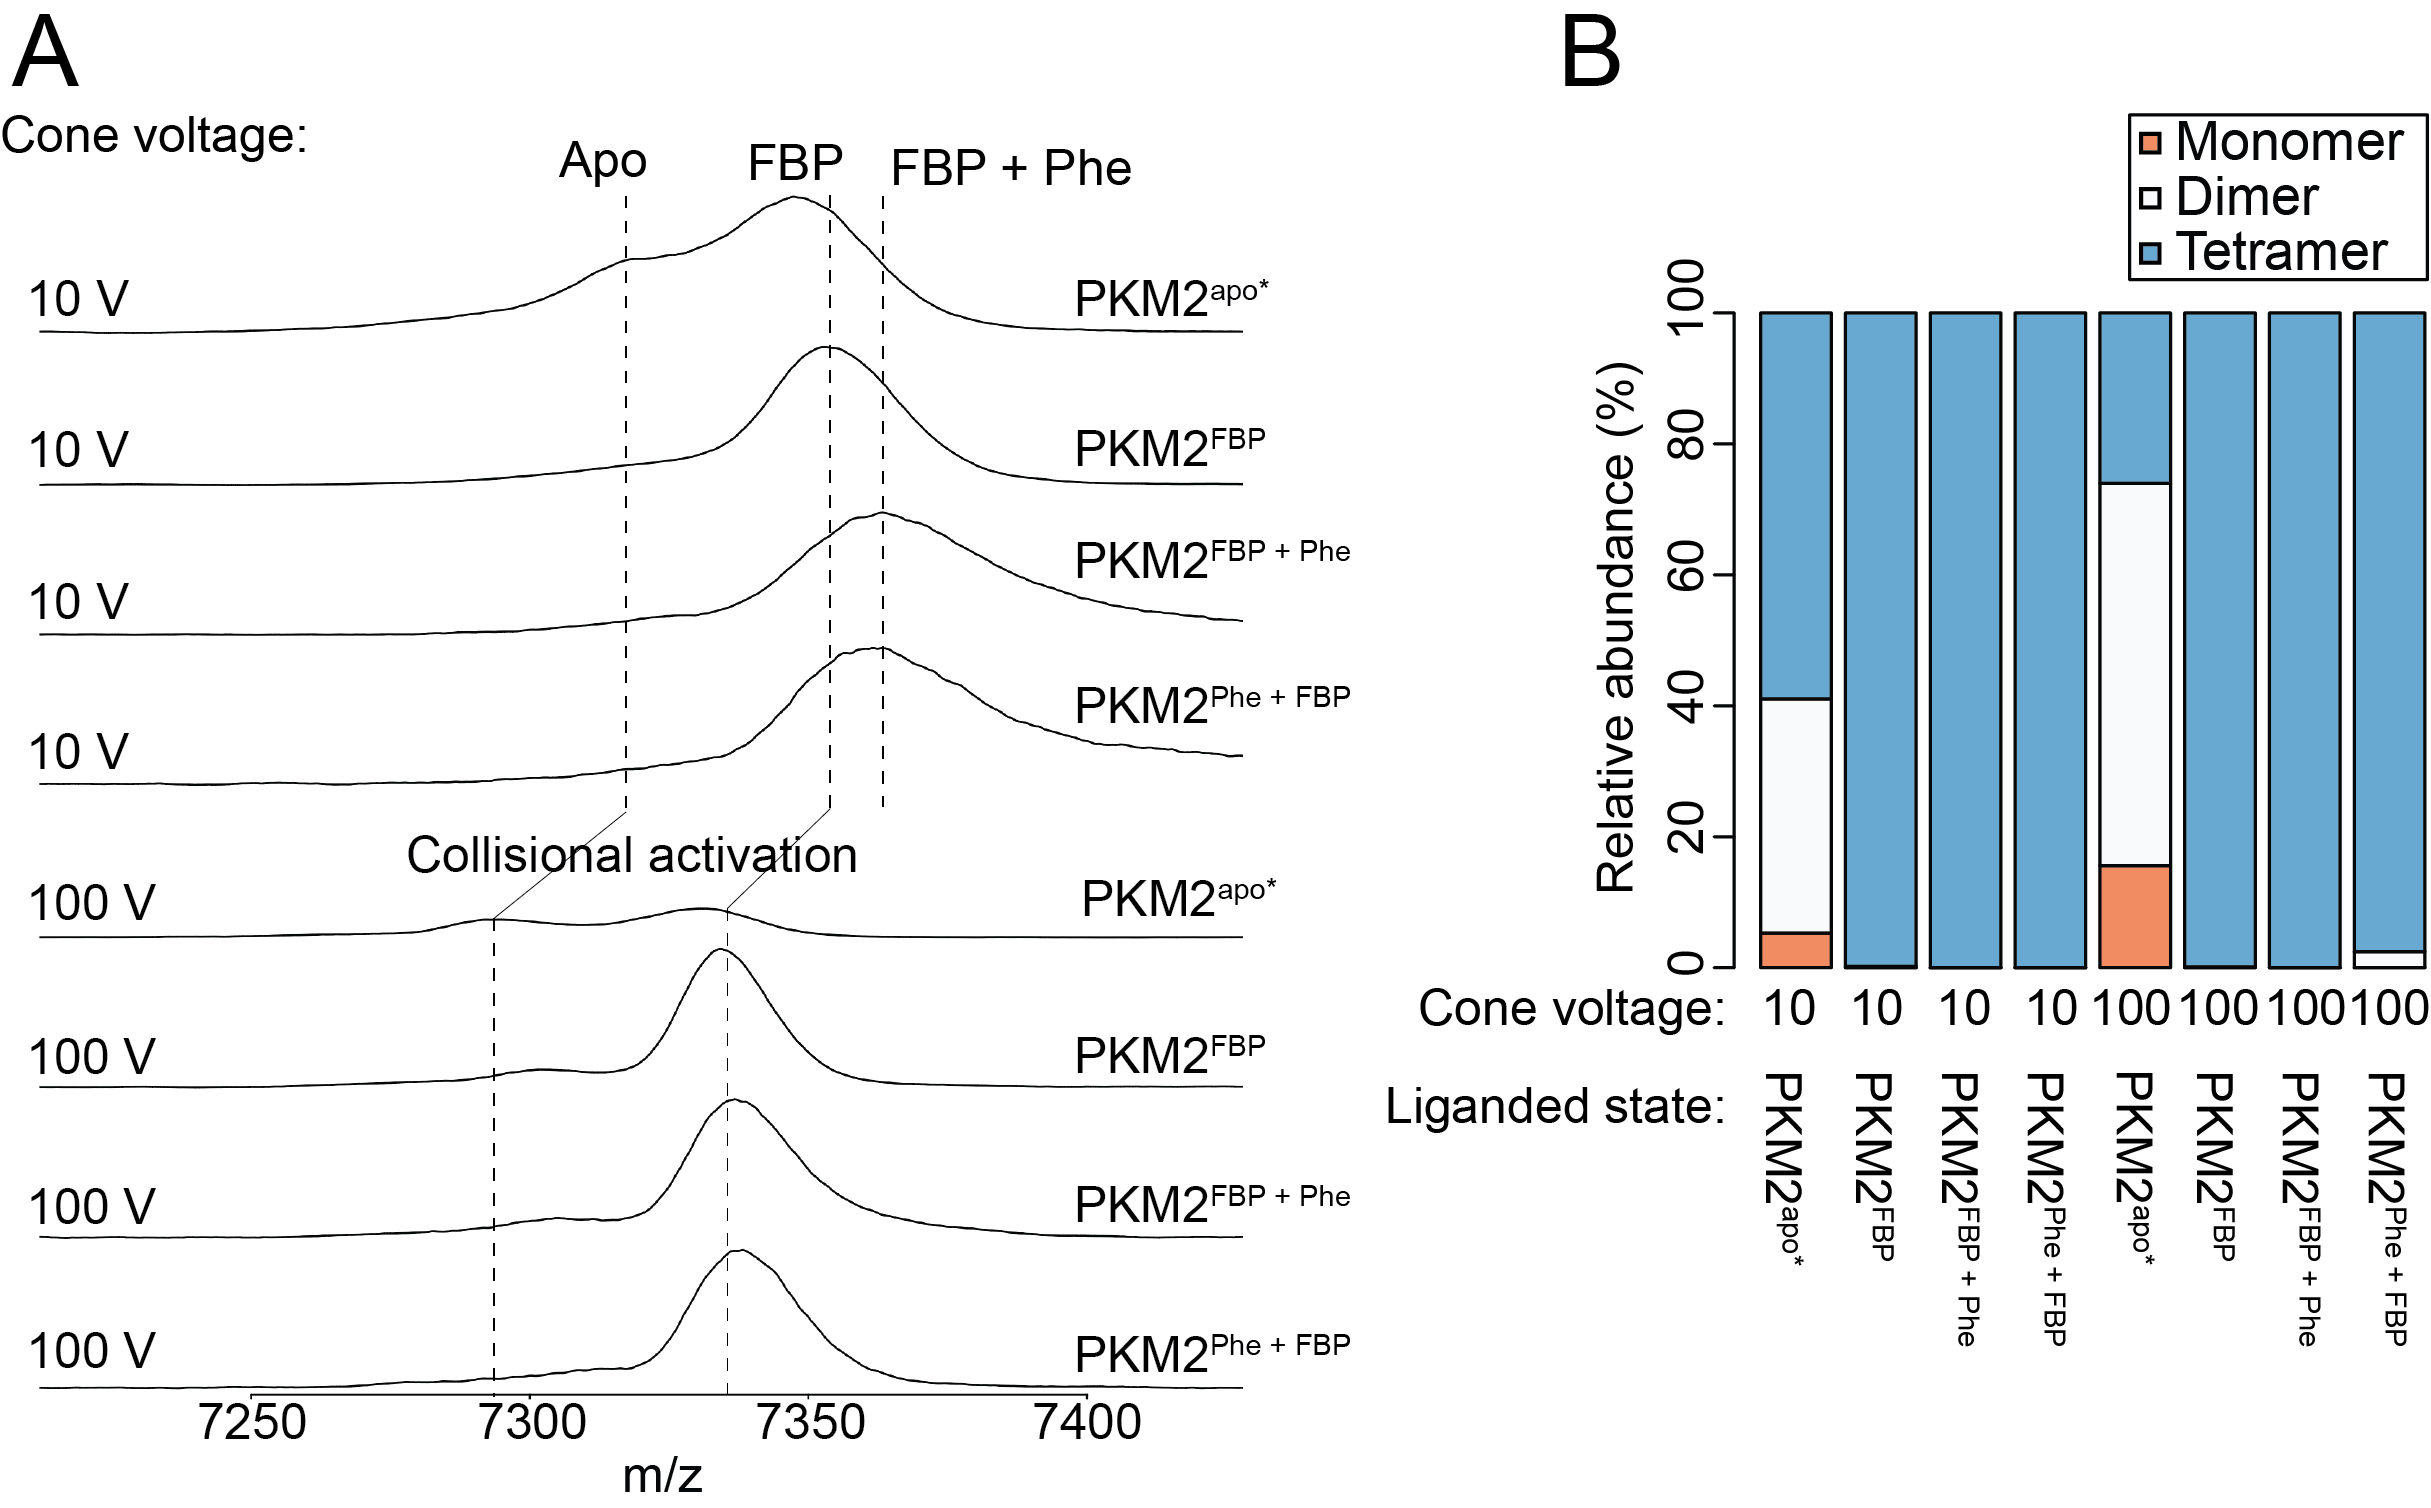
\includegraphics[scale=0.7]{ch5_fig10_fbp_phe_hi_CV_ms.png}
\caption[FBP and Phe can simultaneously bind to PKM2.] {\textbf{FBP and Phe can simultaneously bind to PKM2.} \textbf{(A)} Mass spectra of PKM2 were acquired in the absence of any added ligands (PKM2$^{apo \ast}$), and following the addition of stoichiometric amounts of FBP (PKM2$^{FBP}$); addition of 400 $\mu$M Phe to 10 $\mu$M PKM2 pre-incubated with FBP (PKM2$^{FBP+Phe}$); or addition of 10 $\mu$M FBP to PKM2 pre-incubated with 400 $\mu$M Phe (PKM2$^{Phe+FBP}$). Spectra were acquired with the cone-voltage of the electrospray ionisation source set at either 10 V (native-like) or 100 V (collisional activation). Positions of the m/\textit{z} peaks are shown as dashed lines. \textbf{(B)} The relative abundances of monomer (orange), dimer (white) and tetramer (blue) species were quantified from the spectra in (\textbf{A}).}
\label{fig:fbp_phe_binding_ms}
\end{figure}

\clearpage

\subsection{Phe partially reverses PKM2 to an 'apo-like' conformation}
\label{subsec:ccsd_phe_fbp}
Previous calculations of the CCS (Section \ref{subsec:fbp_ccsd}) revealed subtle conformational changes in PKM2 in response to FBP binding. Given that the subsequent addition of Phe was found to reduce the $\frac{k_{cat}}{K_M}$ ratio to apo-like levels (Chapter \ref{chapter:enzyme_kinetics}) we questioned whether the apparent conformational changes might be predictive of the enzyme activity level of the protein. To this end, IM-MS measurements of PKM2 were repeated following concurrent addition of Phe and FBP. We found that simultaneous binding of Phe and FBP partially reversed the FBP-induced shift towards higher $^{DT}$CCS$_{He}$ values (\textbf{Fig. \ref{fig:fbp_phe_imms}}), suggesting that Phe might reverse the conformational changes associated with FBP-induced enzyme activation.  
%
%
%
%
%%% FIGURE
%
\begin{figure}[!ht]
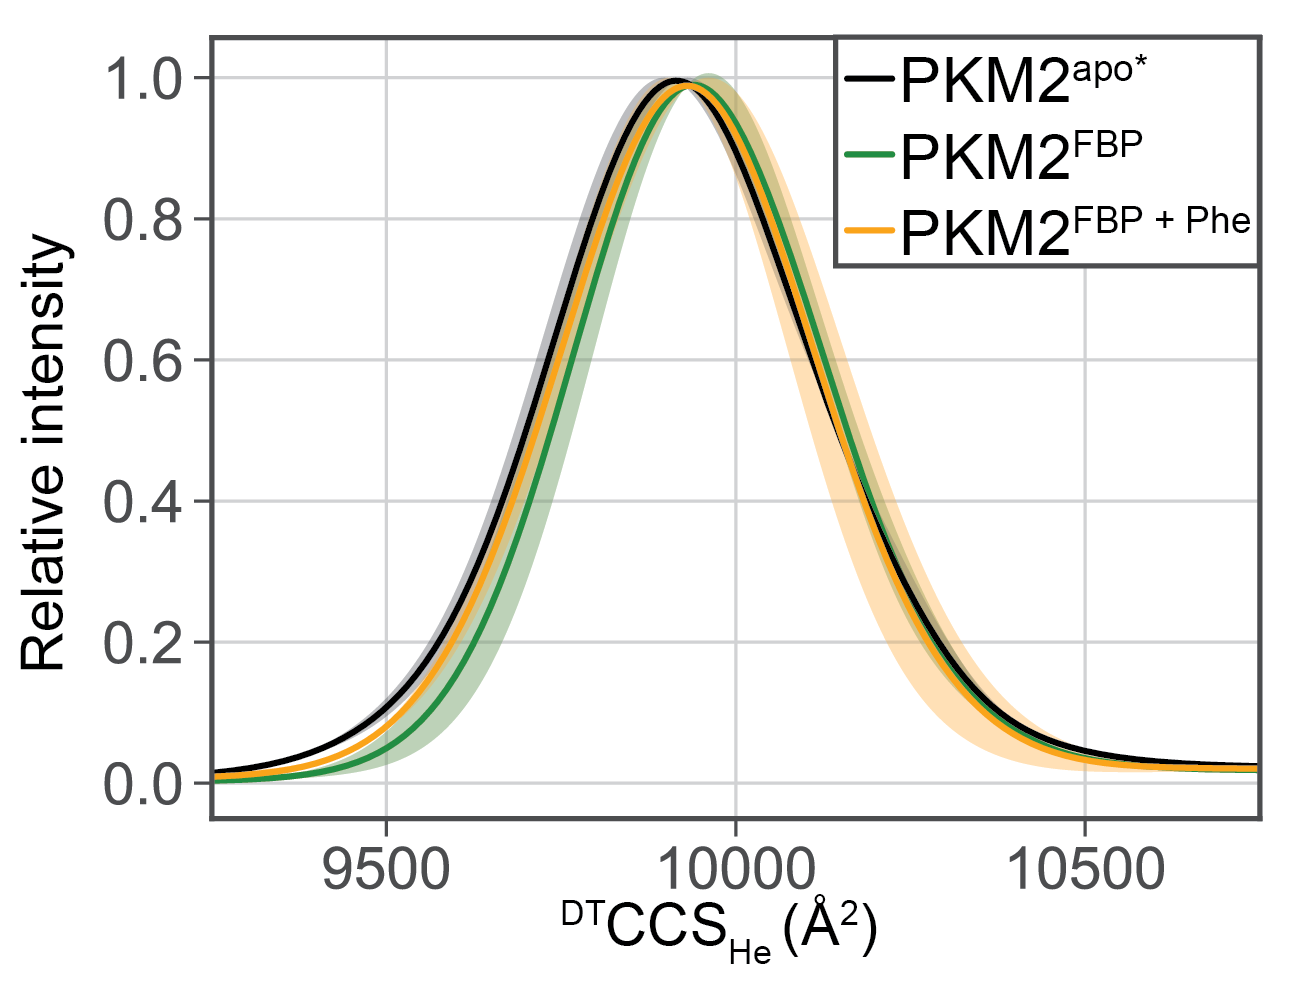
\includegraphics[scale=0.8]{ch5_fig11_fbp_phe_imms.png}
\caption[Phe partially reverses FBP-induced conformational changes.] {\textbf{Phe partially reverses FBP-induced conformational changes.} IM-MS measurements of PKM2 in the absence of any added ligands (black) in the presence of stoichiometric amounts of FBP (green) and in the presence of FBP and 300 $\mu$M Phe (orange). A protein concentration of 10 $\mu$M was used for all measurements.}
\label{fig:fbp_phe_imms}
\end{figure}

\clearpage

 

\section{Conclusion}
Collectively, enzymology, biophysics and native mass spectrometry suggest that allosteric regulators of PKM2 exert distinct effects on PKM2 catalysis by modulating the $K_{M}^{PEP}$ and the $k_{cat}$. Furthermore, this differential effect on alternative aspects of enzyme catalysis is proposed to be routed in the oligomeric structure of PKM2.
%
%
A characterisation of amino acid and FBP binding revealed that the kinetics of ligand binding to these two pockets occcur independently. The binding of amino acids was found to occur with the same apparent dissociation constant irrespective of whether or not FBP is bound to its pocket, and \textit{vice versa}. Concurrent binding of Phe and FBP to PKM2 was further supported by the finding that subsequent ligand addition results in further reversible shifts to the charge-state distribution of PKM2 tetramers. 
\\\\
However, a functional cross-talk between the two binding pockets is proposed. In support of this hypothesis we have found that the enzyme kinetics of PKM2 are distinct when both amino acids and FBP are bound simultaneously, compared to their effects \textit{per se}. Moreover, the functional synergism between amino acid and FBP binding is manifest by enhanced kinetics PKM2 oligomerisation, despite opposing effects of Phe and Ala stabilising dimers and FBP stabilising the tetrameric state. This suggested a functional cross-talk routed in the mechanism of allosteric signal transfer from either allosteric pocket to the protomer interfaces and the active sites, possibly through cooperation between the allosteric pathways connecting these functional sites. 
\\\\
In order to understand the molecular basis of this functional cooperation between amino acid and FBP regulation, we sought to model the effect of these allosteric ligands on the conformational dynamics of PKM2 using molecular dynamics simulations. In addition, we developed a computational method designed to extract allosteric pathways from molecular dynamics simulations in a statistically robust manner.   




















